\subsection{Sensorbaustein}\label{subsec: Sensorbaustein}
\label{sec: Sensorbaustein}
In diesem Unterkapitel werden die Anforderungen und die Hardware des Sensorbausteins behandelt.
Vom Auftraggeber ist ein Sensorbaustein mit 4-Tasten-Feld und Temperaturfühler gefordert. Der Sensorbaustein wird dabei ähnlich einer Unterputzsteckdose montiert und hat eine WLAN-Schnittelle um die Sensordaten auszulesen. In der Abbildung \ref{pic: Uebersicht_Sensorbaustein} ist die Übersicht des Sensorbausteins dargestellt. Der Baustein wird über einAC/DC Wandler der an der Hauselektrik angeschlossen werden kann mit 5V Spannung versorgt. Da der Mikrocontroller auf 3.3V läuft, wird mithilfe eines weiteren Spannungswandlers die 5 V zu 3.3 V gewandelt, so kann auch der USB Anschluss als Spannungsversorgung dienen. Um den Mikrocontroller zu programmieren steht eine USB zu UART Verbindung, Taster zum Debbuggen, Reseten oder Programmieren und eine Zustands-LED zur Verfügung. Um die Temperatur zu erfassen wird ein NTC verwendet. Da die mitgelieferte Meander-Antenne des ESP32 nur eine kleine Abstrahlleistung hat, kann optional noch eine grössere Antenne, wie z.B. eine zertifizierte grössere Patch-Antenne über RP-SMA angeschlossen werden, falls der ESP32S ausgewählt wird. Der Anwender wird ein Touch-Tastenfeld, sowie dazugehörige LEDs, für die Interaktion mit dem Baustein zur Verfügung haben. Zusammenfassend besteht der Sensorbaustein im wesentlichen aus 3 Teilen, nämlich der Spannungsversorgung, der Hauptplatine und der Frontplatte.

\begin{figure}[H]
	\centering
	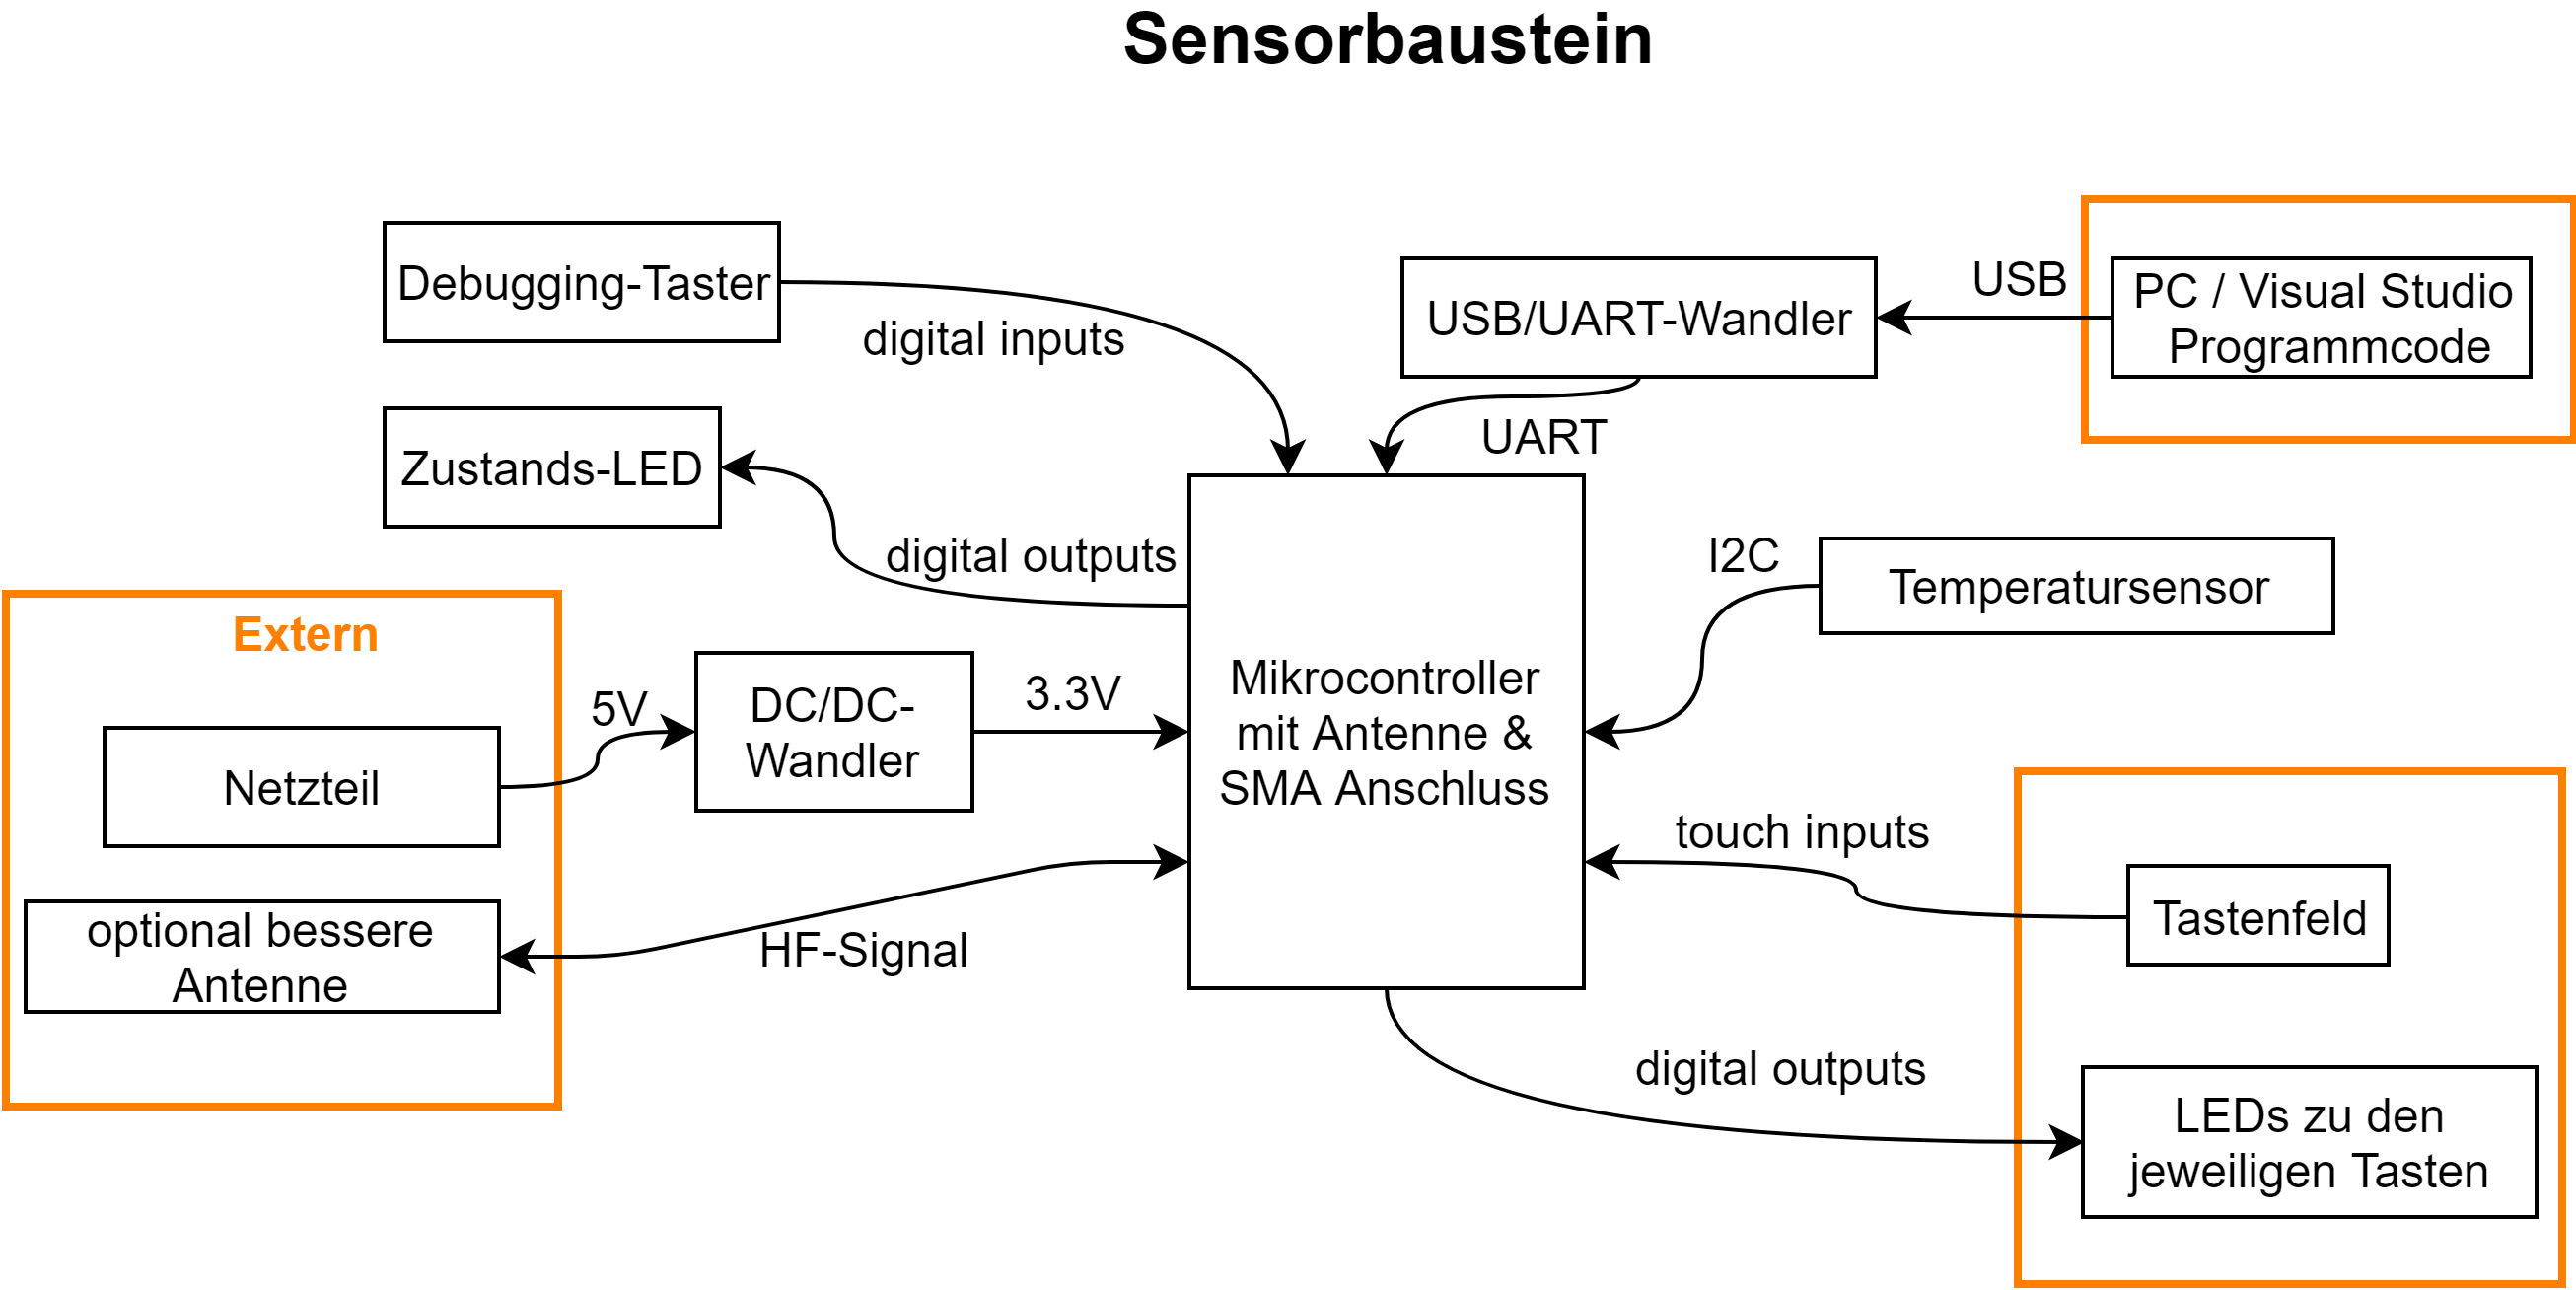
\includegraphics[width=\textwidth]{graphics/Sensorbaustein.png}
	\caption{Übersicht Sensorbaustein}
	\label{pic: Uebersicht_Sensorbaustein}
\end{figure} 

\subsubsection{Übersicht Frontplatte}
Die Frontplatte besteht aus einem 2-Lagen Print. Auf der Vorderseite (Abb. \ref{pic: Frontplatte_vorne}) sind vier runde Kupferflächen angebracht, welche als Touch Fläche fungieren. Wenn nun ein Anwender eine dieser Fläche berührt, wird die Kapazität zwischen dieser Fläche und Ground vergrössert. Natürlich befindet sich ein Lötstopplack zwischen Finger und Kupferfläche der Dielektrikum darstellt. Der ESP32 hat intern Touchsensoren verbaut, welche ein Signal auf auf die Pins geben und dann vermutlich mithilfe eines Spannungsteilers messen ob, dass Signal grösser oder kleiner wird. Zu den Tasten gibt es jeweils eine LED, welche von der Rückseite montiert werden. Der NTC ist auf der Rückseite der Frontplatte angebracht. Um die Temperatur der tatsächlichen Raumluft zu messen wurde auf der Frontplatte eine Kupferfläche auf der Aussenseite angebracht, welche die Wärme via Vias zum NTC weitergibt. Als Verbindung zur Hauptplatine des Sensorbausteins ist ein 12-Pin Stecker mit 2.54\,mm Rastermass vorgesehen. Eine Randnotiz: Es wurde darauf geachtet, dass keine visuell störenden Vias, das optische Erscheinungsbild beeinträchtigen.

\begin{figure}[h!]
	\centering
	\begin{minipage}[t]{0.4\linewidth}
	\centering
	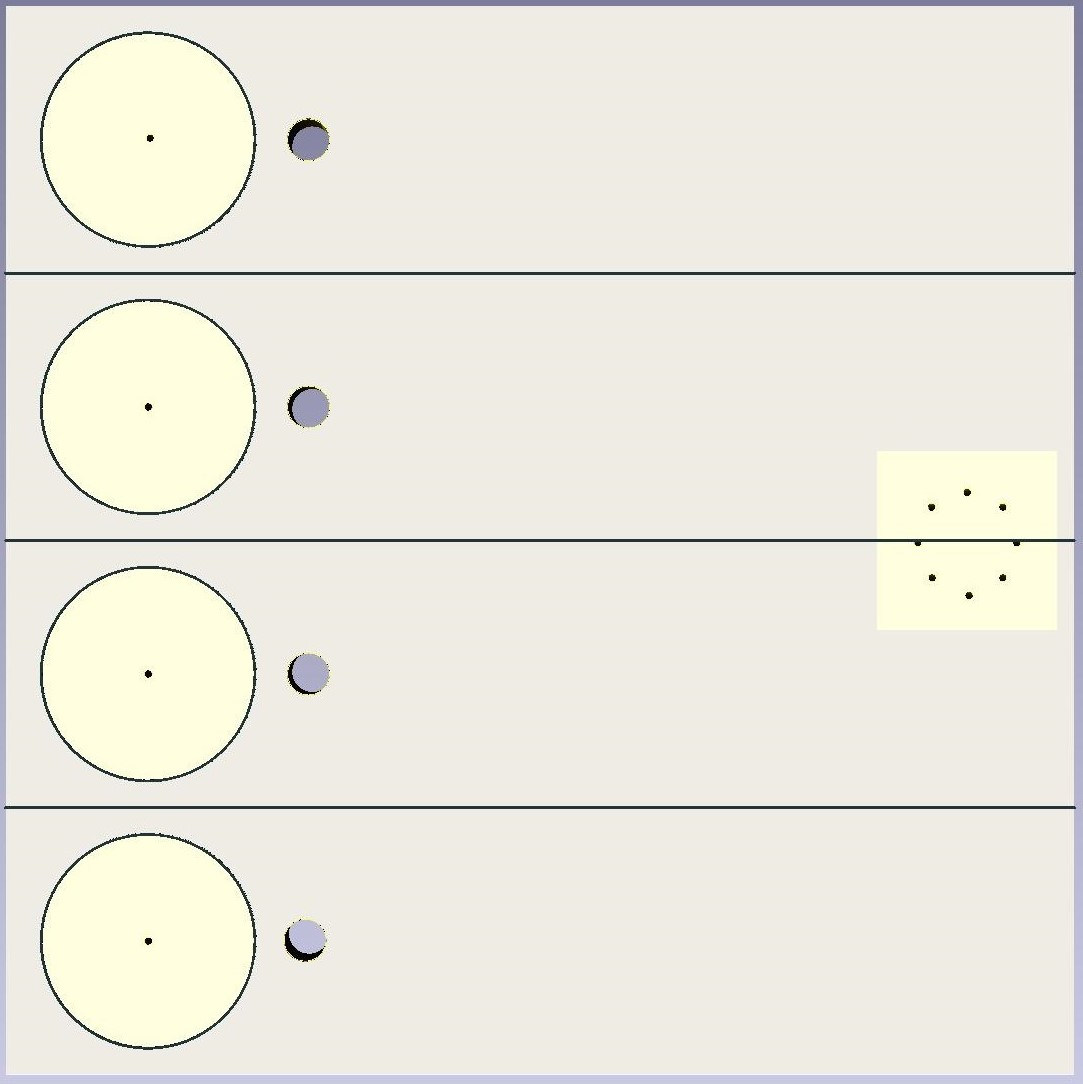
\includegraphics[width=1\textwidth]{graphics/Frontplatte_vorne.jpg}
	\caption{Frontplatte Vordersansicht}
	\label{pic: Frontplatte_vorne}
	\end{minipage}% <- sonst wird hier ein Leerzeichen eingefügt
	\hfill
	\begin{minipage}[t]{0.4\linewidth}
	\centering
	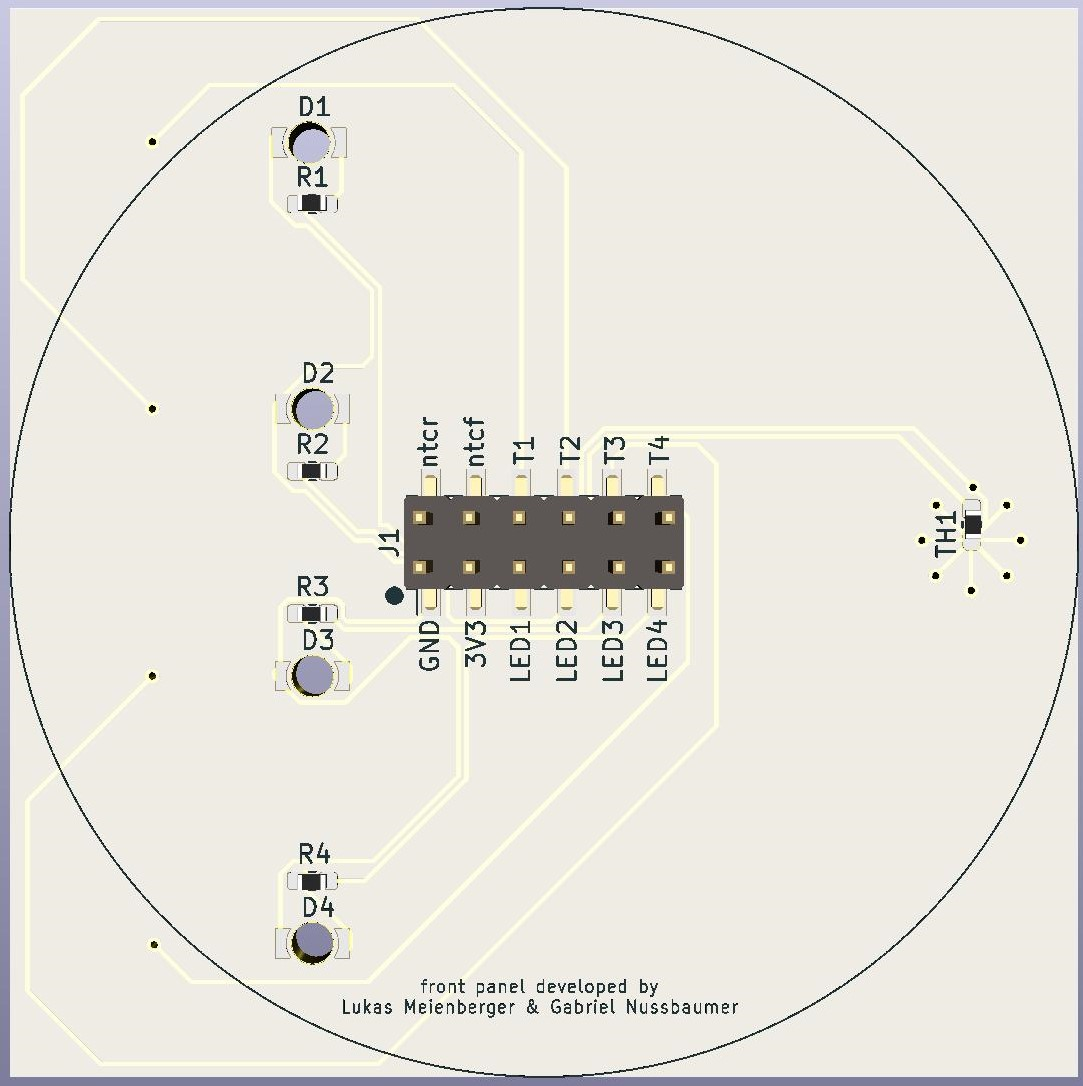
\includegraphics[width=1\textwidth]{graphics/Frontplatte_hinten.jpg}
	\caption{Frontplatte Rückansicht}
	\label{pic: Frontplatte_hinten}
	\end{minipage}
\end{figure}

\subsubsection{Übersicht Hauptplatine}
Auf der Vorderseite der Hauptplatine des Sensorbausteins (Abb. \ref{pic: Hauptplatine_vorne}) befindet sich der ESP32, der Programmieranschluss über USB und den 5V/3V Wandler. Über die Buchse kann dann die Frontplatte angeschlossen werden, wobei auf die Richtung geschaut werden muss. Auf der Rückseite (Abb. \ref{pic: Frontplatte_hinten}) sind Shottky-Dioden, welche bei einem allfälligen ESD auf den Touchflächen greiffen. Ebenso befinden sich dort Buttons, eine Status LED sowie 5V und RX/TX Anschlüsse. Randnotiz: Es wurde darauf geachtet, dass die Leiterbahnen zu den Dioden kürzer sind als, die zu den ADC Eingängen.

\begin{figure}[h!]
	\centering
	\begin{minipage}[t]{0.4\linewidth}
		\centering
		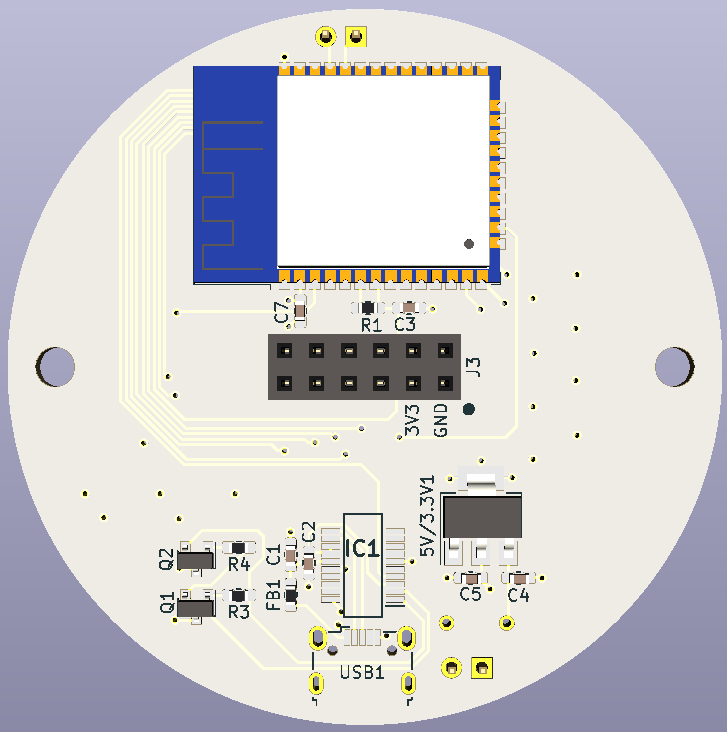
\includegraphics[width=1\textwidth]{graphics/Hauptplatine_vorne.png}
		\caption{Hauptplatine Vorderansicht}
		\label{pic: Hauptplatine_vorne}
	\end{minipage}% <- sonst wird hier ein Leerzeichen eingefügt
	\hfill
	\begin{minipage}[t]{0.4\linewidth}
		\centering
		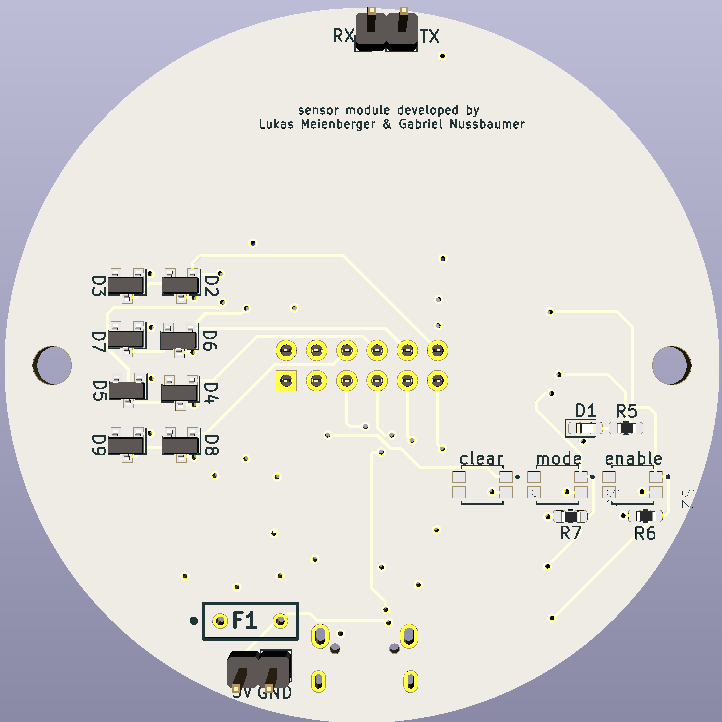
\includegraphics[width=1\textwidth]{graphics/Hauptplatine_hinten.png}
		\caption{Hauptplatine Rückansicht}
		\label{pic: Hauptplatine_hinten}
	\end{minipage}
\end{figure}

\subsubsection{Schutzbeschaltung}

\begin{figure}[h!]
	\centering
	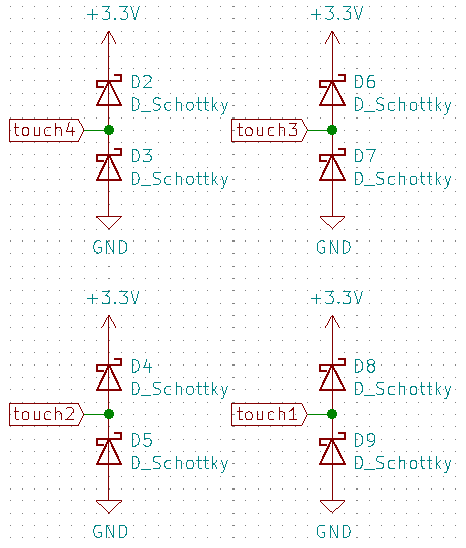
\includegraphics[width=0.4\textwidth]{graphics/shematics_sensor_Shottky.png}
	\caption{Shottky Dioden für ESD Schutz}
	\label{pic: Sensor_Shottky}
\end{figure}


\subsubsection{Mikrocontroller}
\label{Hardware Mikrocontroller_Sensor}
Um die Datenkommunikation über WLAN bereitzustellen wird entweder ein ESP32-WROOM oder der ESP32S, welcher im gleichen Formfaktor zur integrierten Antenne auch einen SMA Anschluss bietet, verwendet. Der ESP32 unterstützt Wi-Fi im Bereich von 2.4 GHz bis ca. 2.5 GHz \cite{espressif_esp32-wroom-32_datasheet_en_2019}. Aus folgender Übersicht sind die zur Verfügung gestellten Ein-/Ausgänge des ESP32 zu entnehmen:
% Please add the following required packages to your document preamble:
% \usepackage{graphicx}
% Please add the following required packages to your document preamble:
% \usepackage{graphicx}
\begin{table}[h!]
	\centering
	\begin{tabular}{|c|c|}
		\hline
		\textbf{Name}                                                                          & \textbf{Anzahl} \\ \hline
		\begin{tabular}[c]{@{}c@{}}Analog-to-Digital Converter (ADC)\\   channels\end{tabular} & 18              \\ \hline
		SPI interfaces                                                                         & 3               \\ \hline
		UART interfaces                                                                        & 3               \\ \hline
		I2C interfaces                                                                         & 2               \\ \hline
		PWM output channels                                                                    & 16              \\ \hline
		Digital-to-Analog Converters (DAC)                                                     & 2               \\ \hline
		I2S interfaces                                                                         & 2               \\ \hline
		Capacitive sensing GPIOs                                                               & 10              \\ \hline
	\end{tabular}
	\caption{I/O Uebersicht}
	\label{tab: IO Uebersicht}
\end{table}
\\
Der ESP32 verfügt über alle benötigten Schnittstellen, die für den Sensorbaustein relevant sind. Im folgenden (Tabelle \ref{tab: IO Sensorbaustein}) sind die Inputs/Outputs des Mikrocontrollers (folglich Abb. \ref{pic: ESP32_sensor}), welcher im Sensorbausteins verwendet wird, aufgeführt:
\begin{table}[h!]
	\centering
	\begin{tabular}{|c|c|}
		\hline
		\textbf{Name}                                                                          & \textbf{Anzahl} \\ \hline
		digital outputs für LEDs                                                               & 5               \\ \hline
		digital inputs für Buttons                                                             & 3               \\ \hline
		\begin{tabular}[c]{@{}c@{}}Capacitive sensing GPIOs für Touch\\   Buttons\end{tabular} & 4               \\ \hline
		UART interface für Programmierung                                                      & 3               \\ \hline
		I2C interfaces für Temperatursensor                                                    & 3               \\ \hline
	\end{tabular}
	\caption{I/O Sensorbaustein}
	\label{tab: IO Sensorbaustein}
\end{table}
\\
\begin{figure}[h!]
	\centering
	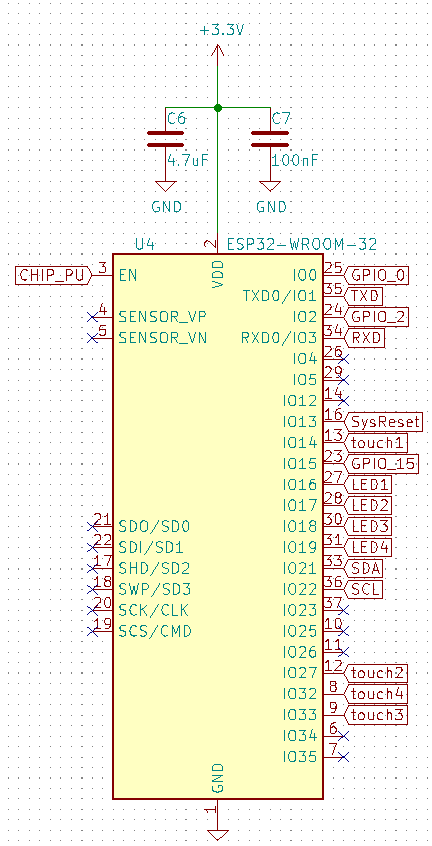
\includegraphics[width=0.4\textwidth]{graphics/shematics_sensor_ESP32.png}
	\caption{Mikrocontroller ESP32 im Sensorbaustein}
	\label{pic: ESP32_sensor}
\end{figure}
\subsubsection{Temperatursensor}
Es wird der NTC NCU18WF104J60RB von Murata Electronics verwendet. Dieser hat den preislichen Vorteil gegenüber anderen Varianten, wie ein Temperaturfühler IC. Der verwendete NTC hat eine B-Konstante von 4250\,K im Bereich 25/50\,°C mit einer Toleranz von 2\%. Der Widerstandswert des NTCs bei 25\,°C beträgt 100\,K mit einer Toleranz von 5\%. Um die Temperatur zu ermitteln wird ein Spannungsteiler (Abb. \ref{pic: Temperatursensor}) ist die verwendete Temperaturschaltung abgebildet. Das Signal ntc $_{ref}$ gibt eine Referenzspannung $U_{ref}$ mithilfe eines DACs aus, da der DAC ungenau ist, wird dieses Signal mithilfe von ntck eingelesen. Die Spannung über dem NTC $U_{ntc}$ wird mit ntcf gemessen und ntcr ist mit Ground verbunden, welches eine separate Rückleitung zur Hauptplatine des Sensorbausteins verfügt, um allfällige Störeinflüsse zu vermeiden. Die Temperatur wird berechnet indem als erstes der Widerstand des NTCs $R_T$ mit $R_T = \frac{U_{ntc}}{U_{ref}\;-\;U_{ntc}}$berechnet wird. Für $U_{ref}$ wird maximal eine Spannung von 2.5\,V verwendet, da der ADC danach nicht mehr linear ansteigt. Dann muss nur noch der ADC Wert mittels einer Geraden in eine Spannung beachtet werden. Die Temperatur in Kelvin ergibt sich dann aus $T = \frac{1}{\frac{1}{T_N}+\frac{1}{B} \cdot ln(R_T)}$.
\begin{figure}[h!]
	\centering
	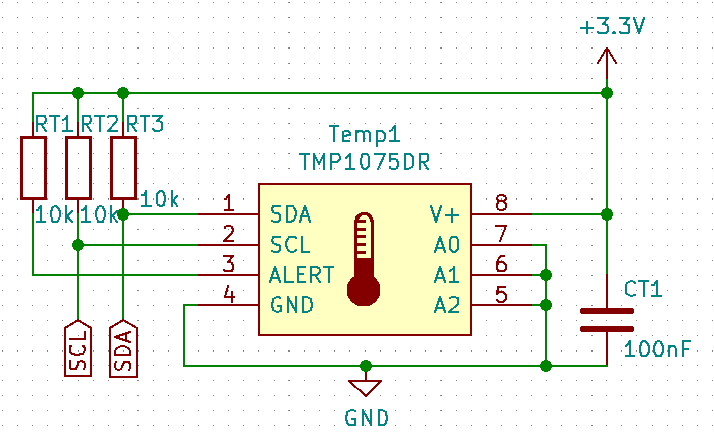
\includegraphics[width=0.4\textwidth]{graphics/shematics_sensor_Temp.png}
	\caption{Schaltung Temperatursensor}
	\label{pic: Temperatursensor}
\end{figure}

\subsubsection{Programmieranschluss}
\label{par: Programmieranschluss}
Der Mikrocontroller kann mittels eines USB to UART Wandlers programmiert werden. Hierzu wird der FT231XS-U verwendet. In Abbildung \ref{pic: USB Anschluss} ist das Schema abgebildet. Auf dem Schema sind dabei zwei Bipolartransistoren zu erkennen, welche es erlauben den ESP32 ohne drücken des Mode- und Enabletasters in den Programmiermodus zu versetzen. Falls es zu Komplikationen kommt steht aber auch die Option mittels des Enable- und Modetaster (Abb. \ref{pic: sensor_progrmmierbuttons}) sich in den Programmiermodus zu versetzen offen. Dazu muss der Modetaster (auch während des ganzen Flashprozesses) gedrückt bleiben, dann mit dem Enabletaster mittels eines kurzen Betätigens den Reset ausgeführt werden und danach kann geflasht werden. Im Aktorbaustein befindet sich die gleiche Schaltung wieder. Falls man einen Systemreset machen möchte kann man den Clear Button betätigen. Die LED5 zeigt mittels eines kurzen Blinkens das Aufstarten des ESP32 an oder oder dass der ESP32 im Programmiermodus ist.
\begin{figure}[h!]
	\centering
	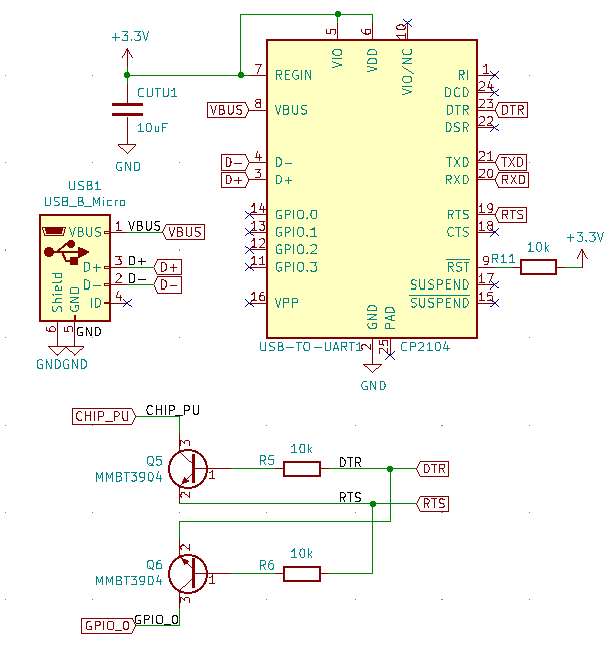
\includegraphics[width=0.7\textwidth]{graphics/shematics_usb.png}
	\caption{USB Anschluss}
	\label{pic: USB Anschluss}
\end{figure}
\begin{figure}[h!]
	\centering
	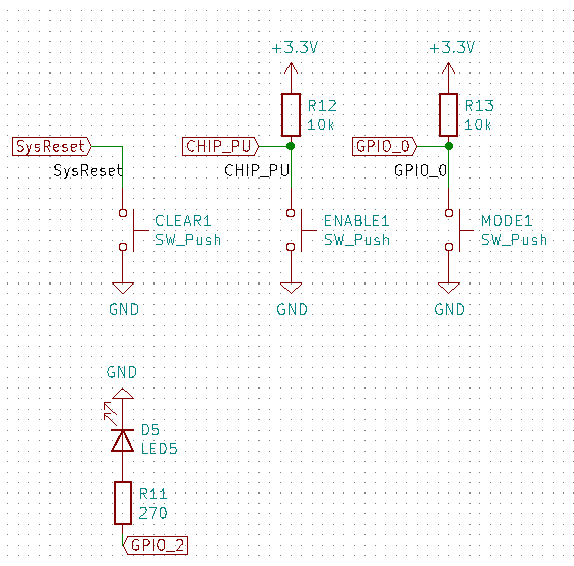
\includegraphics[width=0.4\textwidth]{graphics/shematics_sensor_buttons_LED.png}
	\caption{Buttons und LED auf Sensorbaustein}
	\label{pic: sensor_progrmmierbuttons}
\end{figure}


\subsubsection{Spannungsversorgung}
Der minimale Strom, welche die Spannungsquelle zur Verfügung stellen muss sind laut Datenblatt vom ESP32 500\,mA, wobei im Normalbetrieb 80\,mA und im WiFi Sendebtrieb 160\,mA bis 260\,mA gebraucht werden.
Um den Sensorbaustein mit 5\,V zu versorgen, macht es aus Platz gründen Sinn den 230\,VAC zu 5\,VDC Wandler separat und nicht auf der Hauptplatine zu haben. Dazu wurde der IRM-02-5 verwendet, welcher maximal 2\,W zur Verfügung stellt. Der Mikrocontroller benötigt 3.3\,V, jedoch soll der Sensorbaustein mit 5V betrieben werden können. Hierfür wird einen Spannungswandler eingesetzt. Der ausgewählte AP1117S33CTR hat einen maximale Input Spannung von 15V, eine maximale Dropoutspannung von 1.2\,V bei 800\,mA und ist, mit momentan 0.42\$ bei Digi-Key, günstig. Im Schema (Abb. \ref{pic: Wandler_Sensor}) erkennt man, dass sowohl über USB wie auch über einen Stecker den Print mit 5 V versorgt werden können. Eingebaut ist eine PTC Sicherung sowie eine Diode die verhindern sollen, dass bei einem Kurzschluss oder ähnlichem der Sensorbautein anfängt grossen Schaden zu nehmen.

\begin{figure}[h!]
	\centering
	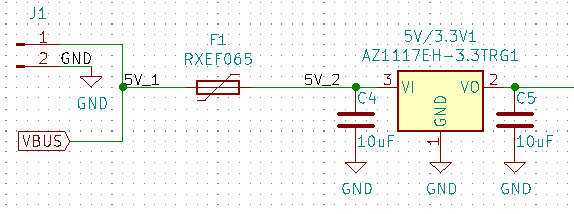
\includegraphics[width=0.5\textwidth]{graphics/shematics_sensor_33V.png}
	\caption{Spannungswandler Sensorbaustein}
	\label{pic: Wandler_Sensor}
\end{figure}

\subsubsection{Platzstudie}
Nun wird mittels einer Platzstudie überprüft ob der Sensorbaustein, mit den verwendeten Komponenten, wie eine Unterputzsteckdose eingebaut werden kann.
Im Bild \ref{pic: Montageplatte.png} ist eine Montageplatte für UP-Steckdosen abgebildet. Der blaue Kreis Zeigt dabei den Radius von 60 mm des Tasters bzw. Kleinkombination. Diese Masse wurden für die Dimensionen der Platine in Abbildung \ref{pic: pcb_sensor_dimensionen.png} übernommen.

\begin{figure}[htb]
	\centering
	\begin{minipage}[t]{0.45\linewidth}
		\centering
		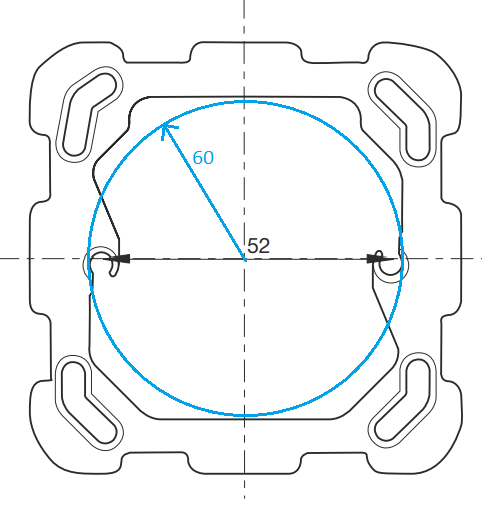
\includegraphics[width=0.9\textwidth]{graphics/Montageplatte.png}
		\caption{Montageplatte \cite{hager_hager_kat1_08_technik_d_2019} }
		\label{pic: Montageplatte.png}
	\end{minipage}% <- sonst wird hier ein Leerzeichen eingefügt
	\hfill
	\begin{minipage}[t]{0.45\linewidth}
		\centering
		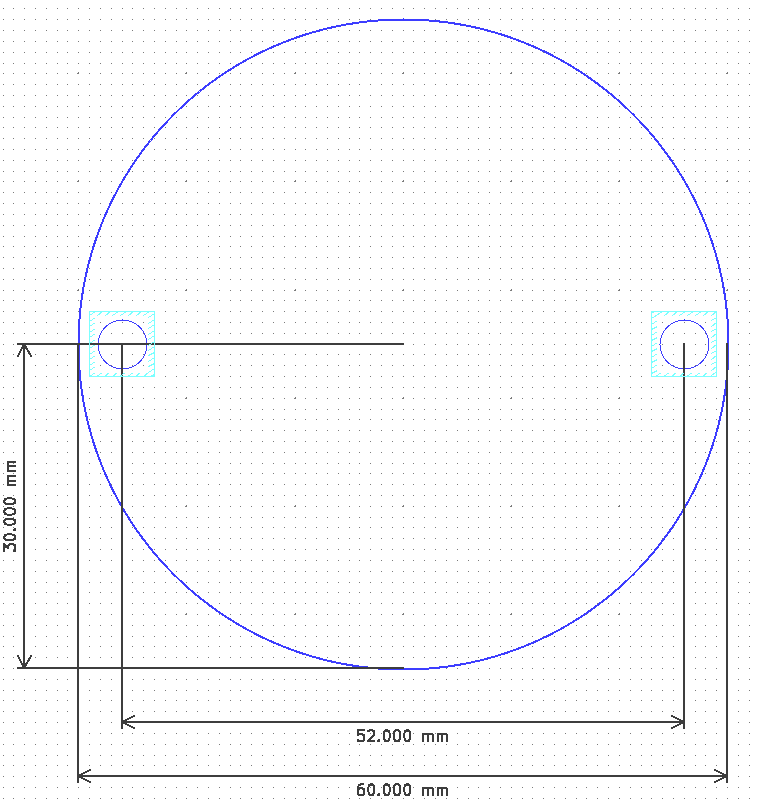
\includegraphics[width=0.90\textwidth]{graphics/pcb_sensor_dimensionen.png}
		\caption{PCB Sensorbaustein Dimensionen}
		\label{pic: pcb_sensor_dimensionen.png}
	\end{minipage}
\end{figure}






